\documentclass[a4paper,11pt]{article} % screen setting

\usepackage[a4paper]{geometry}
\geometry{verbose,tmargin=1.5cm,bmargin=1.5cm,lmargin=1.5cm,rmargin=1.5cm}

\setlength{\parskip}{\smallskipamount}
\setlength{\parindent}{0pt}

%\usepackage{fontspec}
\usepackage[libertine]{newtxmath}
\usepackage[no-math]{fontspec}
\setmainfont{Linux Libertine O}
\setmonofont{DejaVu Sans Mono}

\usepackage{hyperref}
\usepackage{url}
\usepackage{xcolor}

% DARKMODE
%\pagecolor[rgb]{0,0,0} %black
%\color[rgb]{0.8,0.8,0.8} %grey

\usepackage{amsmath}
\usepackage{amssymb}

\usepackage{graphicx}
\usepackage{float}

\usepackage{minted}

\newminted{dart}{breaklines,fontsize=\footnotesize}
\newminted{bash}{breaklines,fontsize=\footnotesize}
\newminted{text}{breaklines,fontsize=\footnotesize}

\newcommand{\txtinline}[1]{\mintinline[breaklines,fontsize=\footnotesize]{text}{#1}}
\newcommand{\dartinline}[1]{\mintinline[breaklines,fontsize=\footnotesize]{python}{#1}}

\newmintedfile[pythonfile]{python}{breaklines,fontsize=\footnotesize}

\definecolor{mintedbg}{rgb}{0.90,0.90,0.90}
\usepackage{mdframed}
\BeforeBeginEnvironment{minted}{
    \begin{mdframed}[backgroundcolor=mintedbg,%
        topline=false,bottomline=false,%
        leftline=false,rightline=false]
}
\AfterEndEnvironment{minted}{\end{mdframed}}


\usepackage{setspace}

\onehalfspacing

\usepackage{appendix}


\newcommand{\highlighteq}[1]{\colorbox{blue!25}{$\displaystyle#1$}}
\newcommand{\highlight}[1]{\colorbox{red!25}{#1}}


\begin{document}


\title{Pemrograman User Interface dengan Flutter:\\
Aplikasi Sederhana dengan Text, Column dan Row}
\author{Fadjar Fathurrahman}
\date{}
\maketitle

\section{Tujuan}

\begin{itemize}
\item Mampu mengenal dan menggunakan baris peritah \txtinline{flutter}
\item Mampu membuat dan membangun project Flutter
\item Mampu membuat program sederhana berbasis \txtinline{StatelessWidget}
\end{itemize}

\section{Baris perintah \txtinline{flutter}}

Dalam praktikum ini kita akan menggunakan baris perintah \txtinline{flutter}
untuk membuat dan membangun project Flutter.

Beberapa perintah yang sering digunakan:

\begin{itemize}
\item \txtinline{flutter create nama_project}: membuat project baru dengan nama
\txtinline{name_project}
\item \txtinline{flutter run -d web}: melakukan testing aplikasi pada web server
\item \txtinline{flutter run -d chrome}: melakukan testing aplikasi pada web server
dan menggunakan browser berbasis Chromium (seperti Google Chrome) untuk
menjalankan aplikasi.
\item \txtinline{flutter run}: menjalankan testing aplikasi pada default target,
biasanya adalah Android atau iOS.
\end{itemize}

\section{Struktur aplikasi Flutter}

Buat project baru dengan \txtinline{flutter}. Misalkan nama project ini
adalah \txtinline{proj_01}:
\begin{textcode}
flutter create proj_01
\end{textcode}

Direktori baru dengan nama \txtinline{proj_01} akan dibuat oleh \txtinline{flutter}
beserta file-file lainnya yang diperlukan.
Struktur dari direktori \txtinline{proj_01} kurang lebih adalah sebagai berikut.

\begin{textcode}
proj_01/
├── android
├── ios
├── lib
│   └── main.dart
├── proj_01.iml
├── pubspec.lock
├── pubspec.yaml
├── README.md
├── test
│   └── widget_test.dart
└── web
\end{textcode}

Kode program Flutter (dalam bahasa pemrograman Dart) akan berada dalam subdirektori
lib.

Buka file \txtinline{lib/main.dart}, hapus semua kode yang ada didalamnya
dan ganti dengan kode berikut.
\begin{dartcode}
import 'package:flutter/material.dart';

void main() {
  runApp(MyApp());
}
  
class MyApp extends StatelessWidget {
  @override
  Widget build(BuildContext context) {
    return MaterialApp(
      title: 'Judul Aplikasi',
      theme: ThemeData(
        primarySwatch: Colors.blueGrey,
        visualDensity: VisualDensity.adaptivePlatformDensity,
      ),
      home: Scaffold(
        appBar: AppBar(title: Text('😍 The AppBar title 😍')),
        body: Text("Hello this is Flutter"),
      )
    );
  }
}
\end{dartcode}

Tampilan aplikasi ketika dijalankan pada web browser kurang lebih seperti
berikut.
\begin{figure}[H]
\centering
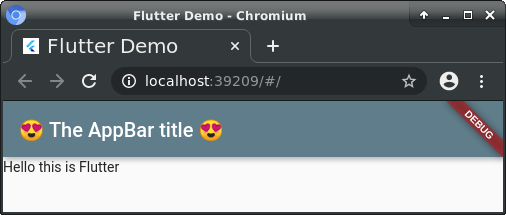
\includegraphics[scale=0.75]{images/flutter_demo_01.png}
\end{figure}


Untuk membuat aplikasi Flutter, kita perlu meng-import beberapa
pustaka standard pada Flutter. Baris berikut ini akan mengimport
elemen-elemen user interface (Material Design, yang dikembangkan
oleh Google) yang digunakan oleh Flutter:
\begin{dartcode}
import 'package:flutter/material.dart';
\end{dartcode}

Seperti pada aplikasi Dart yang lain, fungsi pertama yang akan dijalankan
oleh Flutter adalah fungsi \txtinline{main}.
\begin{dartcode}
void main() {
  runApp(MyApp());
}
\end{dartcode}

Fungsi \txtinline{main} memanggil fungsi \txtinline{runApp()} yang menerima
input berupa \txtinline{Widget}.

Pada Flutter, \txtinline{Widget} dapat dianggap sebagai kelas dasar Flutter
untuk menampilkan user interface. Hampir seluruh kelas atau komponen yang ada
pada Flutter adalah \txtinline{Widget}.

\txtinline{MyApp} adalah sebuah kelas yang kita definisikan sendiri (di luar
pustaka Widget). \txtinline{MyApp} diturunkan (melalui inheritance) dari
kelas \txtinline{StatelessWidget}, yang merupakan kelas dasar \txtinline{Widget}
yang tidak memiliki keadaan atau bersifat statik atau tidak berubah
(\textit{immulatable}).

Semua kelas yang mewarisi atau diturunkan dari \txtinline{Widget} harus
mengimplementasikan fungsi (atau override) \txtinline{build} yang akan mengembalikan
suatu \txtinline{Widget}:
\begin{dartcode}
class MyApp extends StatelessWidget {
  @override
  Widget build(BuildContext context) {
    // Implementasi
  }
}
\end{dartcode}

Kita akan banyak menggunakan pola sebagai berikut untuk
top-level widget yang kita gunakan.
\begin{dartcode}
Widget build(BuildContext context) {
  return MaterialApp(
    title: 'Judul/Nama Aplikasi',
    home: Scaffold(
      appBar: AppBar(title: Text('Judul pada AppBar')),
      body: // Widget Anda di sini,
    )
  );
}
\end{dartcode}


Anda dapat mengganti ukuran font dan font family sebagai berikut.
\begin{dartcode}
Scaffold(
  appBar: AppBar(title: Text('😍 The AppBar title 😍')),
  body: Text("Hello this is Flutter",
    style: TextStyle(fontSize: 40, fontFamily: 'Monaco')
  ),
)
\end{dartcode}


Ganti bagian body dari \txtinline{Scaffold} dengan \txtinline{Column} atau \txtinline{Row}.
Misalnya untuk \txtinline{Column}
\begin{dartcode}
Column(
  children: [
    Text('Teks 1', style: TextStyle(fontSize: 20)),
    Text('Teks 2', style: TextStyle(fontSize: 20)),
    Text('Teks 3', style: TextStyle(fontSize: 30, color: Colors.redAccent),
  ]
)
\end{dartcode}

Kode lengkap untuk file \txtinline{main.dart} menjadi sebagai berikut.
\begin{dartcode}
import 'package:flutter/material.dart';

void main() {
  runApp(MyApp());
}
  
class MyApp extends StatelessWidget {
  // This widget is the root of your application.
  @override
  Widget build(BuildContext context) {
    return MaterialApp(
      title: 'Flutter Demo',
      theme: ThemeData(
        primarySwatch: Colors.blueGrey,
        visualDensity: VisualDensity.adaptivePlatformDensity,
      ),
      home: Scaffold(
        appBar: AppBar(title: Text('😍 The AppBar title 😍')),
        body: Column(children: [
          Text('Teks 1', style: TextStyle(fontSize: 20)),
          Text('Teks 2', style: TextStyle(fontSize: 20)),
          Text('Teks 3', style: TextStyle(fontSize: 30, color: Colors.redAccent)),
        ],),
      )
    );
  }
}
\end{dartcode}

\begin{figure}[H]
{\centering
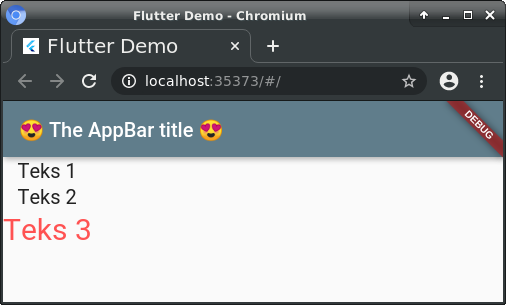
\includegraphics[scale=0.75]{images/flutter_column_01.png}
\par}
\end{figure}

Coba ganti \txtinline{Column} menjadi \txtinline{Row}, apa yang Anda amati?

\section{Tugas}
Buat program sederhana dengan Flutter yang menunjukkan penggunaan
\txtinline{Text} pada gabungan \txtinline{Column} dan \txtinline{Row}.

Beberapa referensi:
\begin{itemize}
\item {\footnotesize\url{https://api.flutter.dev/flutter/widgets/Text-class.html}}
\item {\footnotesize\url{https://api.flutter.dev/flutter/widgets/Row-class.html}}
\item {\footnotesize\url{https://api.flutter.dev/flutter/widgets/Column-class.html}}
\end{itemize}

\bibliographystyle{unsrt}
\bibliography{BIBLIO}

\end{document}
